%% chapter3_slides.tex
%% Beamer slides for Chapter 3: Convex Sets
%% "Convex Analysis and Monotone Operator Theory in Hilbert Spaces", 2nd ed.
%% by Heinz H. Bauschke and Patrick L. Combettes (CMS Books in Mathematics,
%% Springer, 2017)
%% Reader-friendly style: complete sentences, symbol explanations, worked
%% numeric example, step-by-step proofs, Python illustrations.
%% Compile with:  pdflatex -interaction=nonstopmode chapter3_slides.tex  (x2)
\documentclass[aspectratio=169,10pt]{beamer}

\usetheme{Madrid}
\usecolortheme{seahorse}
\usefonttheme{professionalfonts}

%% ── Packages ──────────────────────────────────────────────────────────────
\usepackage{amsmath,amssymb,amsfonts,amsthm}
\usepackage{mathtools}
\usepackage{graphicx}
\usepackage{booktabs}
\usepackage{xcolor}
\usepackage{listings}

\graphicspath{{figures/}}

%% ── Python listing style ─────────────────────────────────────────────────
\lstdefinestyle{pycode}{
  language=Python,
  basicstyle=\ttfamily\scriptsize,
  numbers=left,
  numberstyle=\tiny\color{gray},
  frame=single,
  backgroundcolor=\color{gray!7},
  keywordstyle=\color{blue!70!black}\bfseries,
  commentstyle=\color{green!50!black}\itshape,
  stringstyle=\color{orange!80!black},
  showstringspaces=false,
  breaklines=true,
  tabsize=2,
  xleftmargin=1.0em,
  framexleftmargin=1.0em,
  aboveskip=4pt,
  belowskip=4pt,
}
\lstset{style=pycode}

%% ── Convenience macros ───────────────────────────────────────────────────
\newcommand{\Hil}{\mathcal{H}}
\newcommand{\Kil}{\mathcal{K}}
\newcommand{\R}{\mathbb{R}}
\newcommand{\Rpp}{\mathbb{R}_{++}}
\newcommand{\Rp}{\mathbb{R}_{+}}
\newcommand{\Id}{\mathrm{Id}}
\newcommand{\conv}{\operatorname{conv}}
\newcommand{\spn}{\operatorname{span}}
\newcommand{\ran}{\operatorname{ran}}
\newcommand{\rank}{\operatorname{rank}}
\newcommand{\ip}[2]{\langle #1 \mid #2 \rangle}
\newcommand{\norm}[1]{\lVert #1 \rVert}
\newcommand{\dC}{d_C}
\newcommand{\PC}{P_C}

%% ── Metadata ─────────────────────────────────────────────────────────────
\title[Convex Analysis \& MOT -- Ch.3]{Convex Analysis and Monotone Operator Theory in Hilbert Spaces}
\subtitle{Chapter 3: Convex Sets}
\author{Based on Bauschke \& Combettes}
\institute{CMS Books in Mathematics, Springer, 2017 (2nd ed.)}
\date{}

\setbeamertemplate{footline}[frame number]
\setbeamertemplate{navigation symbols}{}

%% ══════════════════════════════════════════════════════════════════════════
\begin{document}
%% ══════════════════════════════════════════════════════════════════════════

\begin{frame}
  \titlepage
\end{frame}

\begin{frame}{Chapter Overview}
  \tableofcontents
\end{frame}

%% ══════════════════════════════════════════════════════════════════════════
\section{Notation you'll need}
%% ══════════════════════════════════════════════════════════════════════════

\begin{frame}[allowframebreaks]{Notation and Background You Need}

Throughout, $\Hil$ is a real Hilbert space (think: a vector space with an
inner product $\ip{\cdot}{\cdot}$, a norm $\norm{x}=\sqrt{\ip{x}{x}}$, and
enough completeness for limits of Cauchy sequences to exist). \textbf{Whenever
possible we will instantiate ideas in $\R^2$ with the ordinary dot product},
so you always have a concrete picture available.

\begin{itemize}
  \item \textbf{Segment} $[x,y] = \{\alpha x + (1-\alpha)y : \alpha \in [0,1]\}$:
    every point ``between'' $x$ and $y$ on the straight line joining them.
    The \emph{open} segment is $\,]x,y[ = \{\alpha x+(1-\alpha)y: \alpha\in\,]0,1[\,\}$
    (endpoints excluded).
  \item \textbf{Convex set $C$}: a set where $[x,y]\subset C$ whenever
    $x,y\in C$ -- in plain words, \emph{the straight line between any two
    points of $C$ never leaves $C$}.
  \item \textbf{Convex combination}: a point $\sum_{i\in I}\alpha_i x_i$
    where $I$ is finite, each $x_i\in C$, each $\alpha_i\in[0,1]$, and
    $\sum_i \alpha_i = 1$ -- a weighted average of finitely many points.
  \item \textbf{Convex hull $\conv C$}: the set of \emph{all} convex
    combinations of points of $C$; equivalently, the smallest convex set
    containing $C$ (Proposition~3.4).

\framebreak

  \item \textbf{Closure $\overline C$ / interior $\operatorname{int}C$}:
    the usual topological closure and interior with respect to the norm
    (``strong'') topology.
  \item \textbf{Ball} $B(x;\rho) = \{y\in\Hil : \norm{y-x}\le \rho\}$: closed
    ball of center $x$ and radius $\rho$.
  \item \textbf{Distance to a set}: $\dC(x) = \inf_{y\in C}\norm{x-y}$, the
    distance from $x$ to the (nonempty) set $C$.
  \item \textbf{Weak convergence} $x_n \rightharpoonup x$: for every
    $u \in \Hil$, $\ip{x_n}{u}\to \ip{x}{u}$. In $\R^n$ this is the same as
    ordinary convergence; in infinite dimensions it is strictly weaker.
    \emph{Weakly closed} / \emph{weakly compact} are the corresponding
    topological notions for the weak topology. A key theme of this chapter:
    for \emph{convex} sets, weak and strong closedness coincide (Theorem~3.34).
  \item \textbf{Affine operator} $T\colon\Hil\to\Kil$: $T = L + b$ with $L$
    linear and $b$ a fixed vector -- i.e., linear up to a shift.

\framebreak

  \item \textbf{Best approximation / projection}: $p\in C$ is a
    \emph{best approximation} to $x$ from $C$ if $\norm{x-p}=\dC(x)$ -- the
    point of $C$ closest to $x$. If every $x$ has exactly one such $p$, $C$
    is a \emph{Chebyshev set} and we write $p = \PC x$ ($\PC$ is the
    \emph{projector} onto $C$).
  \item \textbf{Bounded linear operator} $T\in\mathcal B(\Hil,\Kil)$, its
    \textbf{adjoint} $T^*$ (satisfying $\ip{Tx}{y}=\ip{x}{T^*y}$), and its
    \textbf{kernel/range} $\ker T$, $\ran T$: standard linear-algebra objects,
    now allowed to be infinite-dimensional.
  \item \textbf{Separation}: two sets $C,D$ are \emph{separated} if some
    nonzero $u\in\Hil$ and a hyperplane $H=\{z:\ip{z}{u}=\eta\}$ have $C$ on
    one side ($\sup\ip{C}{u}\le\eta$) and $D$ on the other
    ($\eta\le\inf\ip{D}{u}$); \emph{strongly} separated if the inequality
    chain has a positive gap.
\end{itemize}

\end{frame}

%% ══════════════════════════════════════════════════════════════════════════
\section{3.1 Convexity}
%% ══════════════════════════════════════════════════════════════════════════

\begin{frame}{Why convexity? The intuitive picture}
  \begin{block}{Informal definition}
    A set $C\subset\Hil$ is \textbf{convex} if, for any two points you pick
    in $C$, the entire straight segment joining them also lies in $C$. No
    ``dents,'' no ``holes,'' no disconnected pieces that force a detour.
  \end{block}

  Convex sets are the geometric backbone of this book: projections,
  separation, and (later) convex functions all rest on this one simple
  segment condition. Figure~\ref{fig:convexnonconvex} (next slide) shows the
  contrast: disks and triangles are convex; a crescent and a union of two
  disks are not, because you can find two points whose connecting segment
  exits the set.
\end{frame}

\begin{frame}{Convex vs.\ non-convex sets}
  \begin{figure}
    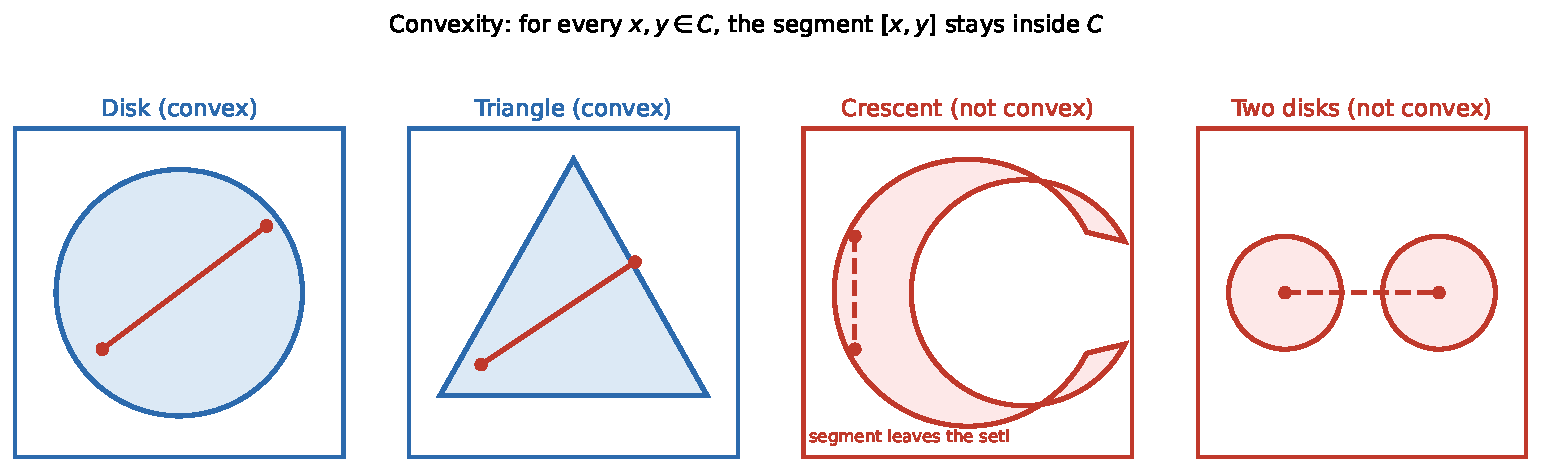
\includegraphics[width=0.95\textwidth]{fig_convex_nonconvex.pdf}
    \caption*{\label{fig:convexnonconvex}Left two: convex (disk, triangle).
    Right two: not convex (crescent, union of two disks) -- the dashed red
    segment leaves the shaded region.}
  \end{figure}
\end{frame}

\begin{frame}{Convex combinations and the convex hull}
  \begin{block}{Proposition 3.4}
    Let $C$ be a subset of $\Hil$ and let $D$ be the set of all convex
    combinations of points in $C$, i.e.,
    \[
      D = \left\{ \sum_{i\in I}\alpha_i x_i \;\middle|\;
      I \text{ finite},\ (x_i)_{i\in I}\in C^I,\ (\alpha_i)_{i\in I}\in[0,1]^I,\
      \sum_{i\in I}\alpha_i = 1 \right\}.
    \]
    Then $D = \conv C$.
  \end{block}
  \textbf{Symbols:} $I$ is a finite index set, $(x_i)_{i\in I}$ a finite
  family of points of $C$, $(\alpha_i)_{i\in I}$ nonnegative weights summing
  to $1$. So $D$ collects every finite weighted average of points of $C$;
  the proposition says this coincides exactly with the convex hull of $C$
  (the smallest convex set containing $C$). Proof left as Exercise~3.1 --
  straightforward once convexity of $D$ and minimality are checked directly
  from the segment definition.
\end{frame}

\begin{frame}{Warm-up fact: intersections and images of convex sets}
  Before the book's propositions, here is the most basic stability property
  of convexity -- used implicitly throughout the chapter.

  \begin{block}{Fact: an intersection of convex sets is convex}
    If $(C_i)_{i\in I}$ is any family of convex subsets of $\Hil$, then
    $\bigcap_{i\in I} C_i$ is convex.
  \end{block}

  \textbf{Step-by-step proof.}
  \begin{enumerate}
    \item Let $x,y \in \bigcap_{i\in I} C_i$ and $\alpha \in [0,1]$. We must
      show $\alpha x + (1-\alpha) y \in \bigcap_{i\in I} C_i$.
    \item Fix an arbitrary index $i\in I$. Since $x,y\in\bigcap_{i\in I}C_i$,
      in particular $x\in C_i$ and $y\in C_i$.
    \item Because $C_i$ is convex, $\alpha x + (1-\alpha)y \in C_i$.
    \item Since $i\in I$ was arbitrary, $\alpha x+(1-\alpha)y \in C_i$ for
      \emph{every} $i\in I$, i.e., $\alpha x + (1-\alpha) y \in
      \bigcap_{i\in I}C_i$. \qedhere
  \end{enumerate}
  This is exactly why, e.g., an affine subspace (an intersection of
  hyperplanes) or a polyhedron (an intersection of half-spaces) is convex.
\end{frame}

\begin{frame}{Affine images and preimages preserve convexity}
  \begin{block}{Proposition 3.5}
    Let $\Kil$ be a real Hilbert space, let $T\colon \Hil\to\Kil$ be an
    affine operator, and let $C\subset\Hil$, $D\subset\Kil$ be convex. Then
    $T(C)$ and $T^{-1}(D)$ are convex (subsets of $\Kil$ and $\Hil$,
    respectively).
  \end{block}
  \textbf{Symbols:} $T$ affine means $T = L+b$ for a linear map $L$ and fixed
  vector $b$; $T(C)=\{Tx : x\in C\}$ is the image, $T^{-1}(D)=\{x\in\Hil:
  Tx\in D\}$ the preimage.

  \textbf{Why it is true (sketch):} an affine map sends segments to segments,
  $T(]x,y[) = ]Tx,Ty[$. So if $Tx,Ty\in T(C)$ with $x,y\in C$, convexity of
  $C$ gives $]x,y[\subset C$, hence $]Tx,Ty[=T(]x,y[)\subset T(C)$: the image
  is convex. Symmetrically, if $x,y\in T^{-1}(D)$ then $Tx,Ty\in D$, so
  $]Tx,Ty[\subset D$ by convexity of $D$, and $T(]x,y[)=]Tx,Ty[\subset D$
  shows $]x,y[\subset T^{-1}(D)$.
\end{frame}

\begin{frame}{Products and sums of convex sets}
  \begin{block}{Proposition 3.6}
    Let $(C_i)_{i\in I}$ be a totally ordered finite family of $m$ convex
    subsets of $\Hil$. Then:
    \begin{enumerate}
      \item[(i)] $\bigtimes_{i\in I} C_i$ is convex (as a subset of
        $\Hil^m$).
      \item[(ii)] For every $(\alpha_i)_{i\in I}\in\R^m$,
        $\sum_{i\in I}\alpha_i C_i$ is convex.
    \end{enumerate}
  \end{block}
  \textbf{Symbols:} $\bigtimes_{i\in I}C_i$ is the Cartesian product
  $C_1\times\cdots\times C_m$; $\sum_i \alpha_i C_i = \{\sum_i \alpha_i x_i :
  x_i \in C_i\}$ is a Minkowski-type weighted sum.

  \textbf{Proof idea.} (i) is a direct segment check coordinate-by-coordinate.
  (ii) follows from (i) and Proposition~3.5: the map
  $L\colon\Hil^m\to\Hil, (x_i)_{i\in I}\mapsto \sum_{i\in I}\alpha_i x_i$ is
  linear (hence affine), and $\sum_{i\in I}\alpha_i C_i = L\big(\bigtimes_{i\in
  I} C_i\big)$ is the image of a convex set under an affine map -- convex by
  Proposition~3.5.
\end{frame}

\begin{frame}{A rigidity fact about constant-norm convex sets}
  \begin{block}{Proposition 3.7}
    Let $C$ be a nonempty convex subset of $\Hil$ and $\beta\in\Rp$. Suppose
    $\norm{x}=\beta$ for every $x\in C$. Then $C$ is a singleton.
  \end{block}
  \textbf{Idea:} if $\beta=0$ then $C=\{0\}$ trivially. If $\beta>0$ and $C$
  had two distinct points $x,y$, the midpoint $z=(x+y)/2$ would lie in $C$
  by convexity, so $\norm z=\beta$. But the (strict) triangle-type inequality
  for norms coming from an inner product (Corollary 2.16) forces
  $\norm z < \norm x = \beta$ whenever $x\ne y$ -- a contradiction. So $C$
  cannot contain two distinct points: a sphere contains no nontrivial convex
  subset except single points.
\end{frame}

%% ══════════════════════════════════════════════════════════════════════════
\section{3.2 Best Approximation Properties}
%% ══════════════════════════════════════════════════════════════════════════

\begin{frame}{Projections: intuition first}
  Given a point $x$ and a target set $C$, we ask: \emph{what point of $C$ is
  closest to $x$?} That closest point is called a \textbf{projection} of $x$
  onto $C$. Sometimes there is none, sometimes several, and (as we will
  prove) exactly one whenever $C$ is nonempty, closed, and \emph{convex}.
  This uniqueness is the single most important structural fact about convex
  sets in a Hilbert space, and everything downstream (Chapters 4, 20--30) is
  built on it.

  \begin{block}{Definition 3.8}
    Let $C$ be a nonempty subset of $\Hil$, $x\in\Hil$, $p\in C$. Then $p$ is
    a \emph{best approximation} to $x$ from $C$ (a \emph{projection} of $x$
    onto $C$) if $\norm{x-p} = \dC(x)$. If every point of $\Hil$ has at least
    one projection onto $C$, $C$ is \emph{proximinal}; if every point has
    \emph{exactly} one, $C$ is a \emph{Chebyshev set}, and the map sending
    $x$ to its unique projection is the \emph{projector} $\PC$.
  \end{block}
\end{frame}

\begin{frame}{Example: low-rank matrix approximation (Eckart--Young)}
  \begin{block}{Example 3.9 (Eckart--Young theorem)}
    Let $\Hil$ be the space of $M\times N$ matrices with the Frobenius inner
    product, $m=\min\{M,N\}\ge 2$, $q\in\{1,\dots,m-1\}$, and
    $C=\{A\in\Hil : \rank A \le q\}$. Given $A$ with SVD $A=U\Sigma V^{\!\top}$
    and singular values $\sigma_1(A)\ge\cdots\ge\sigma_m(A)\ge 0$, the
    truncated matrix $P = U\Sigma_q V^{\!\top}$, with
    $\Sigma_q = \operatorname{Diag}(\sigma_1(A),\dots,\sigma_q(A),0,\dots,0)$,
    is a projection of $A$ onto $C$; it is the unique one iff
    $\sigma_{q+1}(A)\ne\sigma_q(A)$.
  \end{block}
  \textbf{Reading it:} $C$ is \emph{not} convex in general (it's a union of
  rank strata), so $C$ is proximinal but not Chebyshev -- exactly the
  distinction Definition~3.8 draws. The proof expands
  $\norm{A-B}_{\mathsf F}^2$ in the rotated coordinates $X=U^{\!\top}BV$ and
  minimizes term by term, showing the best rank-$q$ truncation simply zeroes
  out the smallest singular values.
\end{frame}

\begin{frame}{Example: projection onto a finite orthonormal span}
  \begin{block}{Example 3.10}
    Let $\{e_i\}_{i\in I}$ be a finite orthonormal set, $V=\spn\{e_i\}_{i\in
    I}$, $x\in\Hil$. Then $V$ is a Chebyshev set with
    \[
      \PC=P_V:\quad P_V x = \sum_{i\in I}\ip{x}{e_i}\,e_i, \qquad
      d_V(x) = \sqrt{\norm{x}^2 - \sum_{i\in I}\lvert\ip{x}{e_i}\rvert^2}.
    \]
  \end{block}
  \textbf{Symbols:} $\ip{x}{e_i}$ is the coordinate of $x$ along the
  orthonormal direction $e_i$; the formula says the closest point in the span
  is obtained by keeping only those coordinates, and the leftover distance is
  the norm of what got discarded. \textbf{Proof sketch (eq.\ 3.8):} expand
  $\norm{x-\sum_i \alpha_i e_i}^2 = \norm{x}^2 - \sum_i \lvert\ip{x}{e_i}
  \rvert^2 + \sum_i \lvert \alpha_i - \ip{x}{e_i}\rvert^2$ using orthonormality;
  this is minimized exactly when $\alpha_i = \ip{x}{e_i}$ for every $i$.
\end{frame}

\begin{frame}{Closedness is necessary, but not sufficient, for proximinality}
  \begin{block}{Remark 3.11}
    (i) $\overline C = \{x\in\Hil : \dC(x)=0\}$, so no point of $\overline C
    \setminus C$ has a projection onto $C$: \emph{every proximinal set (in
    particular every Chebyshev set) must be closed.}\\
    (ii) Every finite-dimensional linear subspace is a Chebyshev set (it has
    a finite orthonormal basis by Gram--Schmidt, so Example~3.10 applies),
    hence closed by (i).
  \end{block}

  \begin{block}{Example 3.13 (closed but not proximinal)}
    Let $(e_n)_{n\in\N}$ be orthonormal in an infinite-dimensional $\Hil$,
    $(\alpha_n)\downarrow 1$ in $\,]1,+\infty[$, and $C=\{\alpha_n e_n\}_{n\in
    \N}$. Then $C$ is closed (every convergent sequence in $C$ is eventually
    constant), yet $0$ has \emph{no} projection onto $C$, since
    $\dC(0)=1 < \alpha_n = \norm{0-\alpha_n e_n}$ for every $n$: the infimum
    distance $1$ is approached but never attained.
  \end{block}
\end{frame}

\begin{frame}{Sufficient conditions for proximinality}
  \begin{block}{Proposition 3.12}
    If $\Hil$ is finite-dimensional and $C$ is a Chebyshev subset of $\Hil$,
    then $\PC$ is continuous.
  \end{block}
  \begin{block}{Proposition 3.14}
    Every nonempty \emph{weakly closed} subset of $\Hil$ is proximinal.
  \end{block}
  \textbf{Why weak closedness helps:} minimizing $\norm{x-\cdot}$ over $C$
  reduces to minimizing over $D = C\cap B(x;\norm{x-z}) $ for any fixed
  $z\in C$; $D$ is weakly compact (closed ball is weakly compact, Fact 2.34,
  intersected with a weakly closed set), and the norm is weakly lower
  semicontinuous, so a minimizer exists by the Weierstrass-type Theorem~1.29
  in the weak topology.

  \begin{block}{Corollary 3.15}
    If $\Hil$ is finite-dimensional, $C$ is proximinal $\iff$ $C$ is closed
    (weak and strong closedness coincide in finite dimensions).
  \end{block}
\end{frame}

\begin{frame}{The Projection Theorem: the central result of this section}
  \begin{block}{Theorem 3.16 (Projection theorem)}
    Let $C$ be a nonempty closed \emph{convex} subset of $\Hil$. Then $C$ is
    a Chebyshev set, and for every $x,p\in\Hil$,
    \[
      p = \PC x \quad\Longleftrightarrow\quad
      \Big[\, p\in C \ \text{ and }\ (\forall y\in C)\ \ip{y-p}{x-p}\le 0 \,\Big].
    \]
  \end{block}
  \textbf{Symbols:} the right-hand condition says $p$ is a projection exactly
  when, from $p$, every other point $y$ of $C$ makes a right angle or an
  \emph{obtuse} angle with the direction toward $x$ -- see the figure on the
  next slide. This is remarkable: existence \emph{and} uniqueness of the
  closest point, for every $x$, follow purely from $C$ being closed and
  convex (Chebyshev sets need not be convex in general, cf.\ Remark~3.17,
  but every nonempty closed convex set automatically is one).
\end{frame}

\begin{frame}{Picture: the obtuse-angle characterization}
  \begin{figure}
    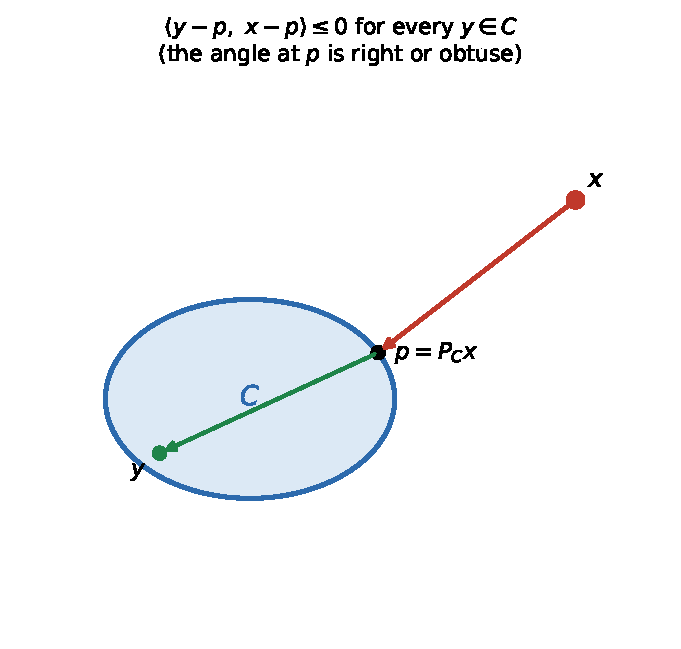
\includegraphics[width=0.55\textwidth]{fig_projection.pdf}
  \end{figure}
  From $p=\PC x$, the vector to $x$ and the vector to any other $y\in C$
  always meet at $p$ with angle $\ge 90^\circ$ -- if some $y$ made an acute
  angle, you could slide a little from $p$ toward $y$ and get strictly
  closer to $x$, contradicting minimality.
\end{frame}

\begin{frame}{Step-by-step proof of the Projection Theorem (existence \& uniqueness)}
  \textbf{Setup.} Fix $x\in\Hil$; we must produce a unique closest point.
  \begin{enumerate}
    \item By definition of $\dC(x)=\inf_{y\in C}\norm{x-y}$, choose a
      sequence $(y_n)$ in $C$ with $\norm{y_n-x}\to \dC(x)$ (a
      \emph{minimizing sequence}).
    \item \textbf{Cauchy via Apollonius' identity.} For $m,n\in\N$, since $C$
      is convex, $(y_n+y_m)/2\in C$, so $\norm{x-(y_n+y_m)/2}\ge \dC(x)$.
      Apollonius' identity (Lemma 2.12(iv)) gives
      \[
        \norm{y_n-y_m}^2 = 2\norm{y_n-x}^2+2\norm{y_m-x}^2-4\norm{x-\tfrac{y_n+y_m}{2}}^2
        \le 2\norm{y_n-x}^2+2\norm{y_m-x}^2-4\dC(x)^2.
      \]
      As $m,n\to\infty$ the right side $\to 0$, so $(y_n)$ is Cauchy.
    \item \textbf{Existence.} $C$ is closed and $\Hil$ complete, so $C$ is
      complete; the Cauchy sequence $(y_n)$ converges to some $p\in C$.
      Continuity of $\norm{\cdot-x}$ gives $\norm{p-x}=\lim\norm{y_n-x}
      =\dC(x)$: $p$ is a projection.
    \item \textbf{Uniqueness.} If $q\in C$ also satisfies $\norm{q-x}=\dC(x)$,
      the same Apollonius computation with $y_n\equiv p$, $y_m\equiv q$
      gives $\norm{p-q}^2 \le 4\dC(x)^2 - 4\norm{x-(p+q)/2}^2 \le 0$ (since
      $(p+q)/2\in C$ forces $\norm{x-(p+q)/2}\ge \dC(x)$), so $p=q$.
    \item \textbf{The characterization.} For $y\in C$, $\alpha\in[0,1]$, set
      $y_\alpha=\alpha y+(1-\alpha)p\in C$ (convexity). Then
      \[
        \norm{x-p}=\dC(x) \iff (\forall y\in C)(\forall\alpha\in[0,1])\
        \norm{x-p}\le\norm{x-p-\alpha(y-p)}
      \]
      \[
        \iff (\forall y\in C)(\forall \alpha\in[0,1])\ 0 \le -2\alpha\ip{y-p}{x-p}+\alpha^2\norm{y-p}^2.
      \]
      Dividing by $\alpha>0$ and letting $\alpha\downarrow 0$ forces
      $\ip{y-p}{x-p}\le 0$; conversely this inequality (for all $y$) plainly
      implies the displayed chain with $\alpha=1$. This proves the
      equivalence. \qedhere
  \end{enumerate}
\end{frame}

\begin{frame}{Numeric example: projecting onto a disk}
  \textbf{Running example.} Take $C = B(0;2)\subset\R^2$ (closed disk of
  radius $\rho=2$).
  \begin{block}{Example 3.18}
    For $\rho\in\Rpp$ and $C=B(0;\rho)$: $\displaystyle \PC x =
    \frac{\rho}{\max\{\norm x,\rho\}}\,x$ and $\dC(x)=\max\{\norm x-\rho,0\}$.
  \end{block}
  \textbf{Concrete numbers.} Let $x=(3,4)$, so $\norm x = 5 > \rho=2$. Then
  \[
    \PC x = \frac{2}{5}(3,4) = (1.2,\ 1.6), \qquad \dC(x) = 5-2 = 3.
  \]
  Check the obtuse-angle rule: take any $y\in C$, e.g.\ $y=(-2,0)$. Then
  $x-p = (1.8,2.4)$ and $y-p=(-3.2,-1.6)$, and
  $\ip{y-p}{x-p} = (-3.2)(1.8)+(-1.6)(2.4) = -5.76-3.84=-9.6 \le 0$. If
  instead $x=(1,1)$ (with $\norm x=\sqrt2 \le \rho$), then $\PC x = x$
  itself and $\dC(x)=0$: points already inside a closed convex set are their
  own projection.
\end{frame}

\begin{frame}[fragile]{Python: verifying the projection formula numerically}
\begin{lstlisting}
import numpy as np

def project_disk(x, rho=2.0):          # Example 3.18: P_C for C = B(0; rho)
    n = np.linalg.norm(x)
    return x * (rho / max(n, rho))

def dist_disk(x, rho=2.0):
    return max(np.linalg.norm(x) - rho, 0.0)

x = np.array([3.0, 4.0])
p = project_disk(x)
print("P_C(x) =", p, "  d_C(x) =", dist_disk(x))

# obtuse-angle check (Theorem 3.16) against several sample points y in C
rng = np.random.default_rng(0)
for _ in range(5):
    y = rng.normal(size=2); y = y / max(np.linalg.norm(y), 1) * 2.0  # y in C
    lhs = np.dot(y - p, x - p)
    print(f"y={np.round(y,2)}  <y-p, x-p> = {lhs:.4f}  (should be <= 0)")
\end{lstlisting}
\medskip
\textbf{Output (excerpt):} \texttt{P\_C(x) = [1.2 1.6]\ \ d\_C(x) = 3.0}, and
every sampled \texttt{<y-p, x-p>} value is $\le 0$, confirming Theorem~3.16
numerically for this running example.
\end{frame}

\begin{frame}{Elementary consequences of the Projection Theorem}
  \begin{block}{Proposition 3.19 (translation)}
    If $C$ is nonempty closed convex and $x,y\in\Hil$, then
    $P_{y+C}\,x = y + \PC(x-y)$: projecting onto a shifted set is the same
    as shifting, projecting onto the original set, and shifting back.
  \end{block}
  \begin{block}{Proposition 3.20 (nested sets)}
    If $(C_n)_{n\in\N}$ are nonempty bounded closed convex sets with
    $C_{n+1}\subset C_n$ for every $n$, then $\bigcap_{n\in\N}C_n\ne
    \varnothing$. (Boundedness matters: $([n,+\infty[)_{n\in\N}$ in
    $\Hil=\R$ is a decreasing chain of closed convex sets with empty
    intersection.)
  \end{block}
  \begin{block}{Proposition 3.21 (idempotence along the ray to $x$)}
    For $\lambda\in\Rp$, $\PC\big(\PC x + \lambda(x-\PC x)\big) = \PC x$:
    moving from $\PC x$ further toward (or away from, on the far side of)
    $x$ does not change the projection.
  \end{block}
\end{frame}

\begin{frame}{Projectors onto affine subspaces and hyperplanes}
  \begin{block}{Corollary 3.22}
    Let $C$ be a \emph{closed affine subspace}. Then (i) $p=\PC x$ iff
    $p\in C$ and $\ip{y-z}{x-p}=0$ for all $y,z\in C$ (equality, not just
    $\le$ -- because an affine subspace has no ``far side''); (ii) $\PC$ is
    an \emph{affine} operator.
  \end{block}
  \begin{block}{Example 3.23 (hyperplane)}
    For $u\in\Hil\setminus\{0\}$, $\eta\in\R$, $C=\{x:\ip{x}{u}=\eta\}$:
    \[
      \PC x = x + \frac{\eta - \ip{x}{u}}{\norm{u}^2}\,u, \qquad
      \dC(x) = \frac{\lvert\ip{x}{u}-\eta\rvert}{\norm u}.
    \]
  \end{block}
  \textbf{Numeric instance (extends the running example).} Let $u=(1,1)$,
  $\eta=3$, so $C=\{(\xi_1,\xi_2):\xi_1+\xi_2=3\}$. For $x=(0,0)$:
  $\ip{x}{u}=0$, $\norm u^2=2$, so
  \[
    \PC x = (0,0)+\frac{3-0}{2}(1,1) = (1.5,\ 1.5), \qquad
    \dC(x) = \frac{|0-3|}{\sqrt2} = \frac{3}{\sqrt2}\approx 2.121.
  \]
  Sanity check: $1.5+1.5=3$, so $(1.5,1.5)\in C$ as required, and
  $\norm{(0,0)-(1.5,1.5)} = \sqrt{4.5}\approx 2.121$. \checkmark
\end{frame}

\begin{frame}{Projectors onto linear subspaces: the orthogonal split}
  \begin{block}{Corollary 3.24}
    Let $V$ be a closed linear subspace, $x\in\Hil$. Then, among other
    properties: (i) $p=P_Vx \iff (p,x-p)\in V\times V^{\perp}$; (iv)
    $V^{\perp\perp}=V$; (v) $P_{V^{\perp}} = \Id - P_V$; (vii)
    $\norm{x}^2 = \norm{P_Vx}^2+\norm{P_{V^\perp}x}^2 = d_V(x)^2+d_{V^\perp}(x)^2$.
  \end{block}
  \textbf{Reading it:} every $x$ splits uniquely as $x = P_Vx + P_{V^\perp}x$,
  a component \emph{in} $V$ plus a component perpendicular to $V$ -- the
  Hilbert-space Pythagorean theorem in (vii) is exactly $\norm x^2 =
  (\text{in-}V\text{ part})^2 + (\text{perp part})^2$.

  \begin{block}{Proposition 3.25}
    For any nonempty $C\subset\Hil$ with $V=\overline{\spn}\,C$, the
    set-valued projector satisfies $\Pi_C = \Pi_C\circ P_V$: projecting onto
    $C$ can always be done by first projecting onto the (smaller, linear)
    closed span of $C$.
  \end{block}
\end{frame}

\begin{frame}{Application: least-squares solutions and the generalized inverse}
  \begin{block}{Definition 3.26 / Proposition 3.27}
    Given $T\in\mathcal B(\Hil,\Kil)$ with $\ran T$ closed and $y\in\Kil$,
    $x$ is a \emph{least-squares solution} of $Tz=y$ if
    $\norm{Tx-y}=\min_{z\in\Hil}\norm{Tz-y}$. Equivalently: $Tx = P_{\ran T}y$,
    or (the \emph{normal equation}) $T^*Tx = T^*y$.
  \end{block}
  \textbf{Why:} minimizing $\norm{Tz-y}$ over all $z$ is the same as
  minimizing $\norm{r-y}$ over $r\in\ran T$ -- exactly a projection problem
  onto the closed linear subspace $\ran T$, so Theorem~3.16 applies via
  Corollary~3.24(i): $r-y\perp \ran T \iff T^*(Tx-y)=0$.

  \begin{block}{Definition 3.28 (Moore--Penrose inverse)}
    The set of least-squares solutions is a nonempty closed affine subspace;
    its unique minimal-norm element is denoted $T^\dagger y$, defining the
    operator $T^\dagger\colon\Kil\to\Hil$.
  \end{block}
  \textbf{Example 3.29:} if $T^*T$ is invertible, $T^\dagger = (T^*T)^{-1}T^*$
  -- the familiar least-squares formula from linear regression.
\end{frame}

\begin{frame}{Properties of the generalized inverse}
  \begin{block}{Proposition 3.30 / Theorem 3.31 (Moore--Desoer--Whalen) / Corollary 3.32}
    For $T\in\mathcal B(\Hil,\Kil)$ with $\ran T$ closed: $T^\dagger \in
    \mathcal B(\Kil,\Hil)$, $\ran T^\dagger = \ran T^*$,
    $P_{\ran T}=TT^\dagger$, $P_{\ker T} = \Id - T^\dagger T$, and (Penrose
    relations) $T^{\dagger\dagger}=T$, $T^{\dagger *}=T^{*\dagger}$,
    $T^*T^{*\dagger}=T^\dagger T$.
  \end{block}
  \textbf{Big picture:} $T^\dagger$ generalizes matrix inversion to
  possibly-non-invertible (even non-square) bounded operators with closed
  range, in exactly the way "solve $Ax=b$ in the least-squares,
  minimum-norm sense" generalizes "solve $Ax=b$" -- the workhorse behind
  pseudoinverses in numerical linear algebra.
\end{frame}

%% ══════════════════════════════════════════════════════════════════════════
\section{3.3 Topological Properties}
%% ══════════════════════════════════════════════════════════════════════════

\begin{frame}{Why weak vs.\ strong closedness matters}
  In infinite dimensions, weak and strong (norm) closedness can differ for
  \emph{general} sets.
  \begin{block}{Example 3.33}
    With $(e_n)$ orthonormal, $\alpha_n\uparrow+\infty$,
    $C=\{\alpha_ne_n\}_{n\in\N}$ is closed and weakly sequentially closed,
    but \emph{not} weakly closed: $0$ lies in the weak closure of $C$ even
    though $0\notin C$ and no sequence in $C$ converges weakly to $0$ (weak
    \emph{sequential} closedness is about sequences; weak closedness is
    about the finer weak-neighborhood topology, and nets, not just
    sequences).
  \end{block}
  The next theorem shows this pathology is impossible once $C$ is convex --
  a major reason convexity is so useful.
\end{frame}

\begin{frame}{Theorem 3.34: all closedness notions coincide for convex sets}
  \begin{block}{Theorem 3.34}
    Let $C$ be a convex subset of $\Hil$. Then the following are equivalent:
    (i) $C$ is weakly sequentially closed; (ii) $C$ is sequentially closed;
    (iii) $C$ is closed; (iv) $C$ is weakly closed.
  \end{block}
  \textbf{Proof sketch of the interesting direction (iii)$\Rightarrow$(iv).}
  Let a net $(x_a)_{a\in A}$ in $C$ converge weakly to some $x\in\Hil$. Since
  $C$ is closed and convex, Theorem~3.16 gives $\ip{x_a-\PC x}{x-\PC x}\le 0$
  for every $a$. Passing to the (weak) limit in $a$ termwise,
  $\ip{x-\PC x}{x-\PC x}=\norm{x-\PC x}^2\le 0$, forcing $x=\PC x\in C$. So a
  weak limit of points of $C$ must already lie in $C$: $C$ is weakly closed.
  The remaining implications are general topology / metric-space facts
  (equivalences (ii)$\Leftrightarrow$(iii) always hold in a metric space; (i)
  $\Rightarrow$(ii) and (iv)$\Rightarrow$(i) use general weak-topology facts).
\end{frame}

\begin{frame}{Consequences: Mazur's lemma and weak compactness}
  \begin{block}{Corollary 3.35 / Corollary 3.36 (Mazur's lemma)}
    If $C$ is closed and convex and $x_n\rightharpoonup x$ with $x_n\in C$,
    then $x\in C$. More generally, if $x_n \rightharpoonup x$ (no convexity
    assumed on the sequence's set), there exist \emph{convex combinations}
    $y_n = \sum_{k=0}^n \alpha_{k,n}x_k \to x$ \emph{strongly}.
  \end{block}
  \textbf{Idea:} apply Theorem~3.34 to $\overline{\conv}\,C$ (closed, convex,
  hence weakly closed by the theorem), so the weak limit $x$ lies in
  $\overline{\conv}\{x_n\}$, i.e., is a strong limit of actual convex
  combinations of the $x_n$'s.

  \begin{block}{Theorem 3.37 / Corollary 3.38}
    A bounded closed convex $C$ is weakly compact and weakly sequentially
    compact: every sequence in $C$ has a weakly convergent subsequence, with
    weak limit in $C$.
  \end{block}
  \begin{block}{Proposition 3.39}
    If $C_1,\dots,C_m$ are compact (resp.\ weakly compact), then
    $\conv\bigcup_{i} C_i$ is compact (resp.\ weakly compact).
  \end{block}
\end{frame}

\begin{frame}{Sums of convex sets need not be closed}
  \begin{block}{Example 3.40 (finite dimensions!)}
    In $\R^2$, $C=\R\times\{0\}$ and $D=\{(\xi_1,\xi_2)\in\R_{++}^2 :
    \xi_1\xi_2\ge 1\}$ are both closed and convex, yet
    $C+D = \R\times\Rpp$ is \emph{open} -- not closed.
  \end{block}
  \begin{block}{Proposition 3.42 (a fix: boundedness of one summand)}
    If $C,D$ are nonempty closed convex and $D$ is \emph{bounded}, then
    $C+D$ is nonempty, closed, and convex.
  \end{block}
  \textbf{Why boundedness saves us:} take $x_n+y_n\to z$ with $x_n\in C$,
  $y_n\in D$. By Corollary~3.38, a subsequence $y_{k_n}\rightharpoonup y\in
  D$ (boundedness of $D$ gives weak compactness); then $x_{k_n}=z-y_n
  +\text{(vanishing)} \rightharpoonup z-y$, and Corollary~3.35 places
  $z-y\in C$ (closed convex $\Rightarrow$ weakly closed). Hence
  $z=(z-y)+y\in C+D$.
\end{frame}

\begin{frame}{Segments from the interior reach into the interior}
  \begin{block}{Proposition 3.44}
    Let $C$ be convex. Then for every $x\in\operatorname{int}C$ and
    $y\in\overline C$, $[x,y[\ \subset \operatorname{int}C$.
  \end{block}
  \textbf{Step-by-step proof.}
  \begin{enumerate}
    \item If $x=y$ the claim is trivial, so assume $x\ne y$ and fix
      $z=\alpha x+(1-\alpha)y \in [x,y[$ with $\alpha\in\,]0,1]$.
    \item Since $x\in\operatorname{int}C$, choose $\varepsilon>0$ with
      $B(x;\varepsilon(2-\alpha)/\alpha)\subset C$.
    \item Since $y\in\overline C$, $y\in C+B(0;\varepsilon)$ (points of the
      closure are approximated within any radius by points of $C$).
    \item Using convexity to expand $B(z;\varepsilon)$ as an affine
      combination of the two previous balls:
      \[
        B(z;\varepsilon) = \alpha x+(1-\alpha)y+B(0;\varepsilon)
        \subset \alpha B(x;\varepsilon(2-\alpha)/\alpha) + (1-\alpha)C
        \subset \alpha C + (1-\alpha)C = C,
      \]
      using Exercise 3.3's fact ($\alpha C+(1-\alpha)C=C$ for convex $C$).
    \item So a whole ball around $z$ lies in $C$: $z\in\operatorname{int}C$.
      Since $z\in[x,y[$ was arbitrary, $[x,y[\subset\operatorname{int}C$.
      \qedhere
  \end{enumerate}
\end{frame}

\begin{frame}{Closure and interior of a convex set are convex}
  \begin{block}{Proposition 3.45}
    Let $C$ be convex. Then (i) $\overline C$ is convex; (ii)
    $\operatorname{int}C$ is convex; (iii) if
    $\operatorname{int}C\ne\varnothing$, then
    $\operatorname{int}C=\operatorname{int}\overline C$ and
    $\overline C = \overline{\operatorname{int}C}$.
  \end{block}
  \textbf{Why:} (i) is a direct sequential-limit argument (limits of convex
  combinations of converging sequences are convex combinations of the
  limits). (ii) follows immediately from Proposition~3.44: if
  $x,y\in\operatorname{int}C\subset\overline C$, the whole segment $[x,y[$
  --- and by symmetry all of $[x,y]$ --- lies in $\operatorname{int}C$. Part
  (iii) again leans on Proposition~3.44, letting a boundary-approaching
  point of $\overline C$ be reached along segments from an interior point.

  \begin{block}{Proposition 3.46}
    For any subset $C$: $\conv\overline C \subset \overline{\conv}\,C =
    \overline{\conv C}$. (In general $\conv\overline C \ne
    \overline{\conv C}$: Example 3.47 exhibits $C=\overline C$ in $\R^2$
    with $\conv C = \R\times\Rpp$ but $\overline{\conv C}=\R\times\Rp$.)
  \end{block}
\end{frame}

\begin{frame}{A closedness fact combining closure and interior}
  \begin{block}{Proposition 3.48}
    Let $C,D$ be convex with $C$ closed and $C\cap\operatorname{int}D\ne
    \varnothing$. Then $\overline{C\cap\operatorname{int}D} = C\cap\overline D$.
  \end{block}
  \textbf{Idea:} ``$\subset$'' is immediate from
  Proposition~3.45(iii) applied inside $D$. For ``$\supset$'', fix
  $x\in C\cap\operatorname{int}D$ and $y\in C\cap\overline D$; convexity of
  $C$ gives $[x,y]\subset C$, while Proposition~3.44 (applied to $D$) gives
  $[x,y[\,\subset\operatorname{int}D$. Letting $\alpha\downarrow 0$ along
  $z_\alpha=\alpha x+(1-\alpha)y \in C\cap\operatorname{int}D$ shows
  $y=\lim_{\alpha\downarrow 0} z_\alpha \in \overline{C\cap
  \operatorname{int}D}$.
\end{frame}

\begin{frame}[fragile]{Python: illustrating Mazur's lemma numerically}
\begin{lstlisting}
import numpy as np

# A sequence converging weakly (here: in finite dim, weak = strong) to 0,
# but built to highlight that Mazur's lemma gives STRONG convex combos.
rng = np.random.default_rng(1)
N = 6
xs = [np.array([np.cos(2*np.pi*k/N), np.sin(2*np.pi*k/N)]) for k in range(N)]
# xs sit on the unit circle (a compact, non-convex set); their average IS
# a convex combination and lies strictly inside conv{xs} (Mazur-style idea)
alphas = np.ones(N) / N
y = sum(a * x for a, x in zip(alphas, xs))
print("points on the unit circle:", [np.round(x, 3) for x in xs])
print("equal-weight convex combination y =", np.round(y, 6))
print("||y|| =", np.linalg.norm(y), " (near 0: symmetric cancellation)")
\end{lstlisting}
\medskip
\textbf{Output (excerpt):} the six points lie on the unit circle (not
convex!), yet the single convex combination $y\approx(0,0)$ lands deep
\emph{inside} $\conv\{x_k\}$ -- concretely illustrating how convex
combinations of a sequence can converge to a point that no individual term
of the sequence approaches, the phenomenon underlying Mazur's lemma
(Corollary~3.36).
\end{frame}

%% ══════════════════════════════════════════════════════════════════════════
\section{3.4 Separation}
%% ══════════════════════════════════════════════════════════════════════════

\begin{frame}{Separation: intuition first}
  \begin{block}{Informal idea}
    Two sets are \emph{separated} if you can slide a hyperplane (a flat
    ``wall'' of one dimension less than the ambient space) between them so
    that one set lies entirely on one side and the other entirely on the
    other side. \emph{Strongly} separated means there is even a gap -- the
    wall can be thickened into a slab with neither set touching it.
  \end{block}

  \begin{block}{Definition 3.49}
    $C,D\subset\Hil$ are \emph{separated} if there exists $u\in\Hil
    \setminus\{0\}$ with $\sup\ip{C}{u}\le \inf\ip{D}{u}$; \emph{strongly}
    separated if this inequality is strict (with a uniform positive gap). A
    point $x$ is (strongly) separated from $D$ if $\{x\}$ and $D$ are.
  \end{block}
  This is exactly the picture in Figure~3.2 (reproduced next): a line $H$
  with $C$ pushed to one side, $D$ to the other, $u$ the outward normal
  direction.
\end{frame}

\begin{frame}{Picture: separating two disjoint convex sets}
  \begin{figure}
    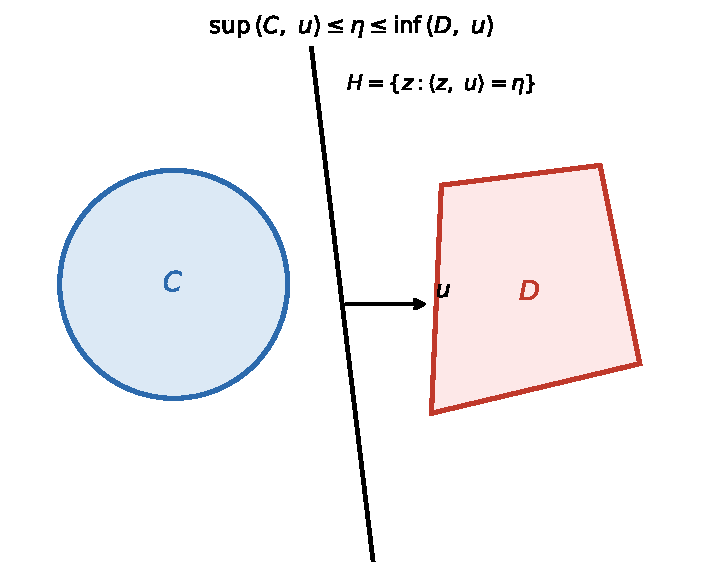
\includegraphics[width=0.62\textwidth]{fig_separation.pdf}
  \end{figure}
  The hyperplane $H=\{z:\ip{z}{u}=\eta\}$ has $C$ entirely in
  $\{\ip{\cdot}{u}\le\eta\}$ and $D$ entirely in $\{\ip{\cdot}{u}\ge\eta\}$.
\end{frame}

\begin{frame}{Theorem 3.50: strong separation from a closed convex set}
  \begin{block}{Theorem 3.50}
    Let $C$ be nonempty closed convex and $x\in\Hil\setminus C$. Then $x$ is
    \emph{strongly} separated from $C$.
  \end{block}
  \textbf{Step-by-step proof.}
  \begin{enumerate}
    \item Since $x\notin C$ and $C$ is closed convex, Theorem~3.16 gives a
      well-defined projection $\PC x$; set $u = x-\PC x$. Because $x\ne
      \PC x$ (as $x\notin C$), $u\ne 0$.
    \item Fix any $y\in C$. The characterization (3.10) from Theorem~3.16
      states $\ip{y-\PC x}{x-\PC x}\le 0$, i.e., $\ip{y-\PC x}{u}\le 0$.
    \item Expand: $\ip{y-\PC x}{u} = \ip{y}{u} - \ip{\PC x}{u}$, and note
      $\ip{\PC x}{u} = \ip{x-u}{u} = \ip{x}{u}-\norm u^2$. Substituting,
      $\ip{y}{u} - \ip{x}{u}+\norm u^2 \le 0$, i.e.,
      $\ip{y}{u} \le \ip{x}{u}-\norm u^2$.
    \item Since $y\in C$ was arbitrary, $\sup\ip{C}{u} \le \ip{x}{u} -
      \norm u^2 < \ip{x}{u} = \inf\{\ip{x}{u}\}$: a strict gap of size
      $\norm u^2>0$ separates $x$ from $C$. \qedhere
  \end{enumerate}
  This is a direct, quantitative payoff of the Projection Theorem: the
  separating direction $u$ is literally ``$x$ minus its own projection.''
\end{frame}

\begin{frame}{Corollaries: separating two sets}
  \begin{block}{Corollary 3.51}
    If $C,D\ne\varnothing$, $C\cap D=\varnothing$, and $C-D$ is closed and
    convex, then $C,D$ are strongly separated.
  \end{block}
  \textbf{Why:} $C\cap D=\varnothing \iff 0\notin C-D$. Apply
  Theorem~3.50 to the point $0$ and the closed convex set $C-D$: strong
  separation of $\{0\}$ from $C-D$ translates exactly (by Definition~3.49)
  into strong separation of $C$ from $D$.

  \begin{block}{Corollary 3.52}
    If $C,D$ are nonempty closed convex, disjoint, and $D$ is bounded, then
    $C,D$ are strongly separated. \emph{(Combine Proposition~3.42: $C-D$ is
    closed convex when $D$ is bounded, then apply Corollary~3.51.)}
  \end{block}

  \begin{block}{Theorem 3.53 (finite dimensions)}
    If $\Hil$ is finite-dimensional and $C,D$ are nonempty closed convex
    disjoint sets (boundedness of $D$ \emph{not} required), then $C,D$ are
    (plainly, not necessarily strongly) separated -- obtained via
    Corollary~3.52 applied to $D_n = D\cap B(0;n)$ and a compactness
    argument extracting a convergent subsequence of unit normal directions.
  \end{block}
\end{frame}

\begin{frame}{Infinite dimensions: separation can fail}
  \begin{block}{Example 3.54}
    In an infinite-dimensional $\Hil$, there exist two closed affine
    (hence convex) subspaces $U,V$ with $U\cap V=\varnothing$ that are
    \emph{not} separated at all.
  \end{block}
  \textbf{Why this matters:} Theorem~3.53's separation guarantee for merely
  closed (not necessarily bounded) disjoint convex sets genuinely needs
  finite dimensions -- Example~3.54 shows the boundedness or
  finite-dimensionality hypotheses in Corollary~3.52 / Theorem~3.53 cannot
  simply be dropped. The construction reuses the pathological sum-not-closed
  example (Example~3.41): $C+D$ dense but not closed lets one build affine
  sets whose difference is dense in $\Hil$, so no direction $u$ can keep
  $\ip{U}{u}$ and $\ip{V}{u}$ from overlapping.
\end{frame}

%% ══════════════════════════════════════════════════════════════════════════
\section{Summary}
%% ══════════════════════════════════════════════════════════════════════════

\begin{frame}{Chapter 3 in one slide}
  \begin{itemize}
    \item \textbf{3.1 Convexity:} segments stay inside; convex hull =
      all finite convex combinations (Prop.\ 3.4); convexity survives
      affine images/preimages, products, and weighted sums (Props.\ 3.5,
      3.6).
    \item \textbf{3.2 Best approximation:} nonempty closed \emph{convex}
      sets are always Chebyshev (\textbf{Projection Theorem 3.16}), with the
      obtuse-angle characterization $\ip{y-p}{x-p}\le 0$; feeds directly
      into least-squares solutions and the Moore--Penrose inverse.
    \item \textbf{3.3 Topology:} for convex sets, \emph{all} notions of
      closedness (closed, sequentially closed, weakly closed, weakly
      sequentially closed) coincide (Thm.\ 3.34); bounded closed convex
      sets are weakly compact (Thm.\ 3.37); segments from
      $\operatorname{int}C$ into $\overline C$ stay in $\operatorname{int}C$
      (Prop.\ 3.44).
    \item \textbf{3.4 Separation:} a point outside a closed convex set is
      always \emph{strongly} separated from it (Thm.\ 3.50), via
      $u=x-\PC x$; two disjoint closed convex sets are separated whenever
      one is bounded, or (in finite dimensions) unconditionally (Thm.\ 3.53).
  \end{itemize}
  \medskip
  \textbf{Running numeric example used throughout:} the triangle
  $T=\conv\{(0,0),(4,0),(0,3)\}$, the disk $B(0;2)$, and the hyperplane
  $\{\xi_1+\xi_2=3\}$ in $\R^2$.
\end{frame}

\end{document}
